\appendix
\renewcommand{\thechapter}{B} % Set Appendix Chapter Label to B

\chapter{MỘT SỐ LỖI THƯỜNG GẶP}
\label{Appendix2}

Phần này bao gồm một số lỗi thường gặp và cách khắc phục trong quá trình triển khai và gỡ lỗi hệ thống Nios V với DMA.

\section{Lỗi Tạo BSP hoặc Biên dịch Ứng dụng}
\label{sec:trouble_bsp_app}

Một lỗi phổ biến khi chạy lệnh \texttt{niosv-app} là báo không tìm thấy tệp hoặc thư mục nguồn (Hình \ref{fig:03_67}).
\begin{itemize}
    \item \textbf{Nguyên nhân:} Đường dẫn đến thư mục \texttt{app}, \texttt{bsp}, hoặc tệp mã nguồn C (\texttt{-s=...}) không chính xác so với vị trí hiện tại (hoặc không tồn tại) của Nios V Shell. 
    \item \textbf{Khắc phục:} Đảm bảo đã \texttt{cd} vào thư mục gốc của dự án Quartus (\texttt{DMANiosVIntern}) trước khi chạy lệnh \texttt{niosv-app}. Kiểm tra lại các đường dẫn tương đối (\texttt{software/app}, \texttt{software/bsp}) trong lệnh. Tên tệp mã nguồn C trong thư mục \texttt{app} phải khớp với tên được chỉ định bởi tham số \texttt{-s}.
\end{itemize}

\begin{figure}[htbp]
    \centering
    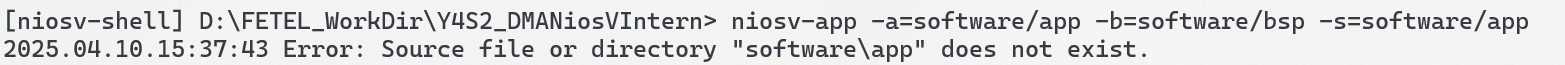
\includegraphics[width=\linewidth]{Images/03_67_AppendixTroubleshootingBSPError.png}
    \caption{Lỗi niosv-app báo đường dẫn hoặc tệp source code không tồn tại.}
    \label{fig:03_67}
\end{figure}

\section{Sự cố Kết nối JTAG và Debug}
\label{sec:trouble_jtag}

Giao tiếp \acrshort{jtag} có thể bị treo hoặc không ổn định, dẫn đến các vấn đề như:
\begin{itemize}
    \item Quartus Programmer không nhận diện được bo mạch DE10-Standard.
    \item Ashling IDE không thể kết nối với Nios V core khi Debug.
    \item Cửa sổ \texttt{juart-terminal} không hiển thị output hoặc không phản hồi.
    \item Không thể tải tệp \acrshort{elf} lên bộ xử lý.
\end{itemize}
\textbf{Khắc phục:}
\begin{itemize}
    \item \textbf{Kiểm tra kết nối vật lý:} Đảm bảo cáp USB-Blaster được kết nối chắc chắn giữa PC và bo mạch.
    \item \textbf{Khởi động lại JTAG Server:} Dịch vụ Altera JTAG Server chạy nền trên Windows có thể bị lỗi. Khởi động lại nó thông qua Task Manager -> Services (tìm "Altera JTAG Server" hoặc "JTAGServer") hoặc dùng lệnh \texttt{jtagconfig --stopserver} và \texttt{jtagconfig --startserver} trong Command Prompt. Có thể cần quyền Administrator. (Xem Hình \ref{fig:A2} để khởi động lại từ Services).
    \item \textbf{Kiểm tra Driver USB-Blaster:} Đảm bảo driver cho USB-Blaster đã được cài đặt đúng cách. Kiểm tra trong Device Manager của Windows.
    \item \textbf{Đóng các ứng dụng khác:} Đảm bảo không có instance nào khác của Quartus Programmer, Ashling IDE, hoặc juart-terminal đang cố gắng truy cập vào kết nối JTAG cùng lúc.
\end{itemize}

\begin{figure}[htbp]
    \centering
    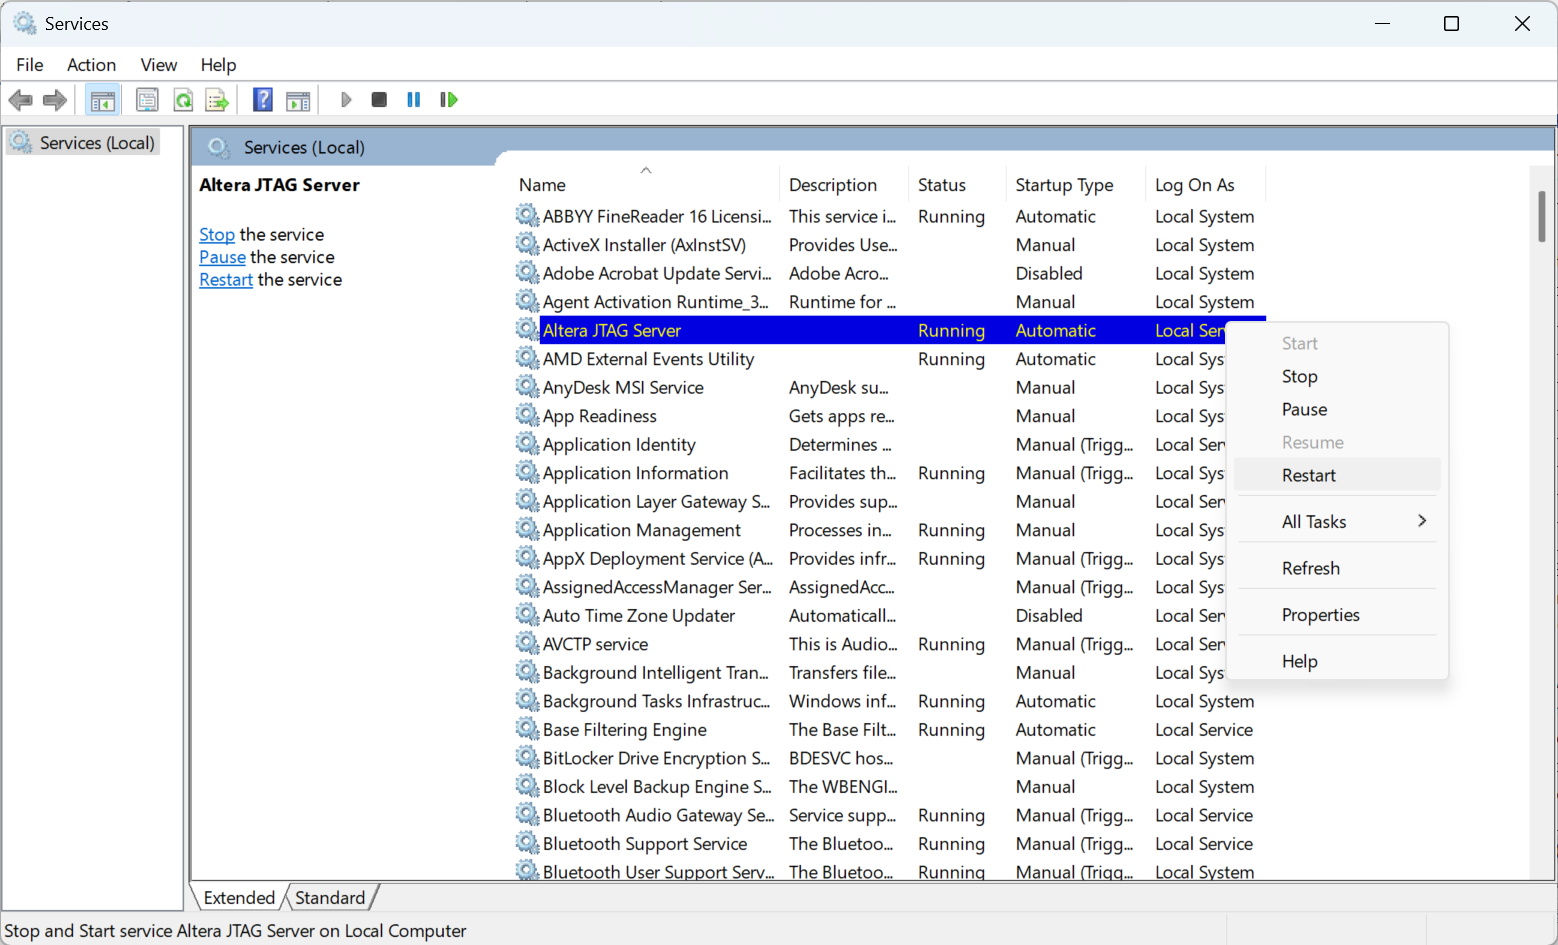
\includegraphics[width=\linewidth]{Images/03_69_AppendixRestartJTAGServer.png}
    \caption{Khởi động lại Altera JTAG Server trong Services của Windows.}
    \label{fig:A2}
\end{figure}

\section{Không có file `.sof` để nạp xuống board}
Nếu gặp lỗi khi tạo tệp `.sof` (liên quan đến biên dịch thất bại), hãy kiểm tra lại trạng thái giấy phép Nios V/m trong Quartus License Setup (Tham khảo Mục \ref{sec:get_license}). Đôi khi giấy phép hết hạn hoặc cấu hình sai có thể gây lỗi biên dịch, gián tiếp ảnh hưởng đến debug. Cộng đồng Intel cũng lưu ý việc phê duyệt tài khoản license có thể mất vài ngày \cite{intel-forum-license}.

\section{Nên sử dụng bản Quartus nào khi xây dựng hệ thống Nios V}
\label{sec:quartus_edition}

Khi làm việc trên Nios II, người dùng có xu hướng dùng bản Quartus 18.x vì tính ổn định, cũng như không cần phải cài thêm WSL1 và tự cài thủ công Eclipse cho Nios II.

Tuy nhiên, trái ngược với Nios II đã ra mắt từ năm 2000, Nios V chỉ mới ra mắt từ năm 2021, và tài liệu đầu tiên của Intel cung cấp cho Nios V là cho nền tảng Quartus 21.3. Lúc này Intel chỉ cung cấp một bản Nios V/m duy nhất. Mãi đến gần giữa 2023 với sự ra mắt của Quartus 23.1 thì đây cũng là lần đầu tiên xuất hiện Nios V/g. Không lâu sau đó thì Nios V/c cũng được ra mắt trên bản Quartus 23.3. Tuy nhiên thì từ đó cho đến hiện tại Intel vẫn liên tục cập nhật các thông tin kỹ thuật, thay đổi các tập lệnh, cũng như đánh giá về mặt phần cứng của Nios V. \cite{niosv-embedded-history}

Chính vì vậy, cách khuyến khích tốt nhất để dùng \acrshort{niosv} đó là nên sử dụng bản Quartus mới nhất để được cập nhật đầy đủ các tính năng, cũng như sửa lỗi cho trình IDE Ashling, và ưu tiên dùng phiên bản theo thứ tự từ cao đến thấp là Pro, Standard rồi đến Lite Edition. Một số lỗi như lỗi tạo Testbench trên Platform Designer khi làm việc trên hệ điều hành Windows chỉ gặp khi sử dụng bản Lite. Có 2 giải pháp để không bị lỗi này đó là chuyển sang bản Standard hoặc Pro (vẫn dùng Windows), hoặc chuyển sang Linux (vẫn dùng bản Lite).

Ngoài ra cũng cần phải chú ý là từ các bản về sau, bộ Quartus chuyển sang dùng Questa Sim (trước kia là ModelSim). Questa Sim cần phải có License để có thể sử dụng. Các bước lấy License cho Questa Sim cũng tương tự như cho \acrshort{niosv} \ref{sec:get_license}.

% \section{Lấy Giấy phép (License) \acrshort{niosv}/m}
\section{Lấy Giấy phép (License) \texorpdfstring{\acrshort{niosv}}{Nios V}/m}
\label{sec:get_license} % Add label for potential cross-referencing

Bộ xử lý \acrshort{niosv}, cụ thể là phiên bản vi điều khiển (microcontroller) \acrshort{niosv}/m được sử dụng trong dự án này, yêu cầu một tệp giấy phép miễn phí (license file) từ Intel để có thể tạo ra các tệp lập trình nạp xuống board (`.sof`) trong phần mềm Quartus Prime. 

\begin{enumerate}
    \item \textbf{Đăng ký Tài khoản:} Truy cập Intel FPGA \acrfull{sslc} \url{https://licensing.intel.com/psg/s/} (Hình \ref{fig:03_01}). 
    \item \textbf{Đăng nhập và Chọn Giấy phép:} Sau khi tài khoản được kích hoạt, đăng nhập (Hình \ref{fig:03_02}) và chọn tùy chọn "Sign up for Evaluation or No-Cost Licenses" (Hình \ref{fig:03_03}).
    \item \textbf{Chọn Nios V/m:} Chọn bộ xử lý "Nios V/m" từ danh sách \acrshort{ip}/phần mềm có sẵn (Hình \ref{fig:03_04}).
    \item \textbf{Thông tin Máy chủ (Host):} Cung cấp chi tiết cho máy tính sẽ sử dụng giấy phép. Chọn "FIXED" cho Loại Giấy phép (License Type) và "NIC ID" cho Loại Máy tính (Computer Type). Nhập Tên Máy tính (Computer Name) mong muốn. Quan trọng là tìm Địa chỉ Vật lý (Physical Address - \acrshort{mac} Address) của thẻ giao diện mạng (network interface card - \acrshort{nic}) của bạn (ví dụ: sử dụng lệnh \texttt{ipconfig /all} trong Windows Command Prompt, Hình \ref{fig:03_05}) và nhập nó vào trường "Primary Computer ID", loại bỏ mọi dấu gạch nối hoặc dấu hai chấm (Hình \ref{fig:03_06}).
    \item \textbf{Tạo Giấy phép:} Đồng ý với các điều khoản và tạo giấy phép (Hình \ref{fig:03_07}).
    \item \textbf{Nhận và Lưu Giấy phép:} Tệp giấy phép (ví dụ: \texttt{LR-XXXXXXXX\_License.dat}) sẽ được gửi qua email (Hình \ref{fig:03_08}). Lưu tệp `.dat` này vào một vị trí thích hợp trên máy tính của bạn.
    \item \textbf{Cấu hình Quartus:} Trong Quartus Prime, điều hướng đến Tools -> License Setup... (Hình \ref{fig:03_09}). Trong cửa sổ License Setup, duyệt đến và chọn tệp giấy phép `.dat` đã tải xuống (Hình \ref{fig:03_10}). Với giấy phép được thêm thành công, Quartus sẽ có thể tạo các tệp lập trình `.sof` cần thiết trong quá trình biên dịch (compile).
\end{enumerate}

% Figure environments for Section 3.1
\begin{figure}[htbp] \centering 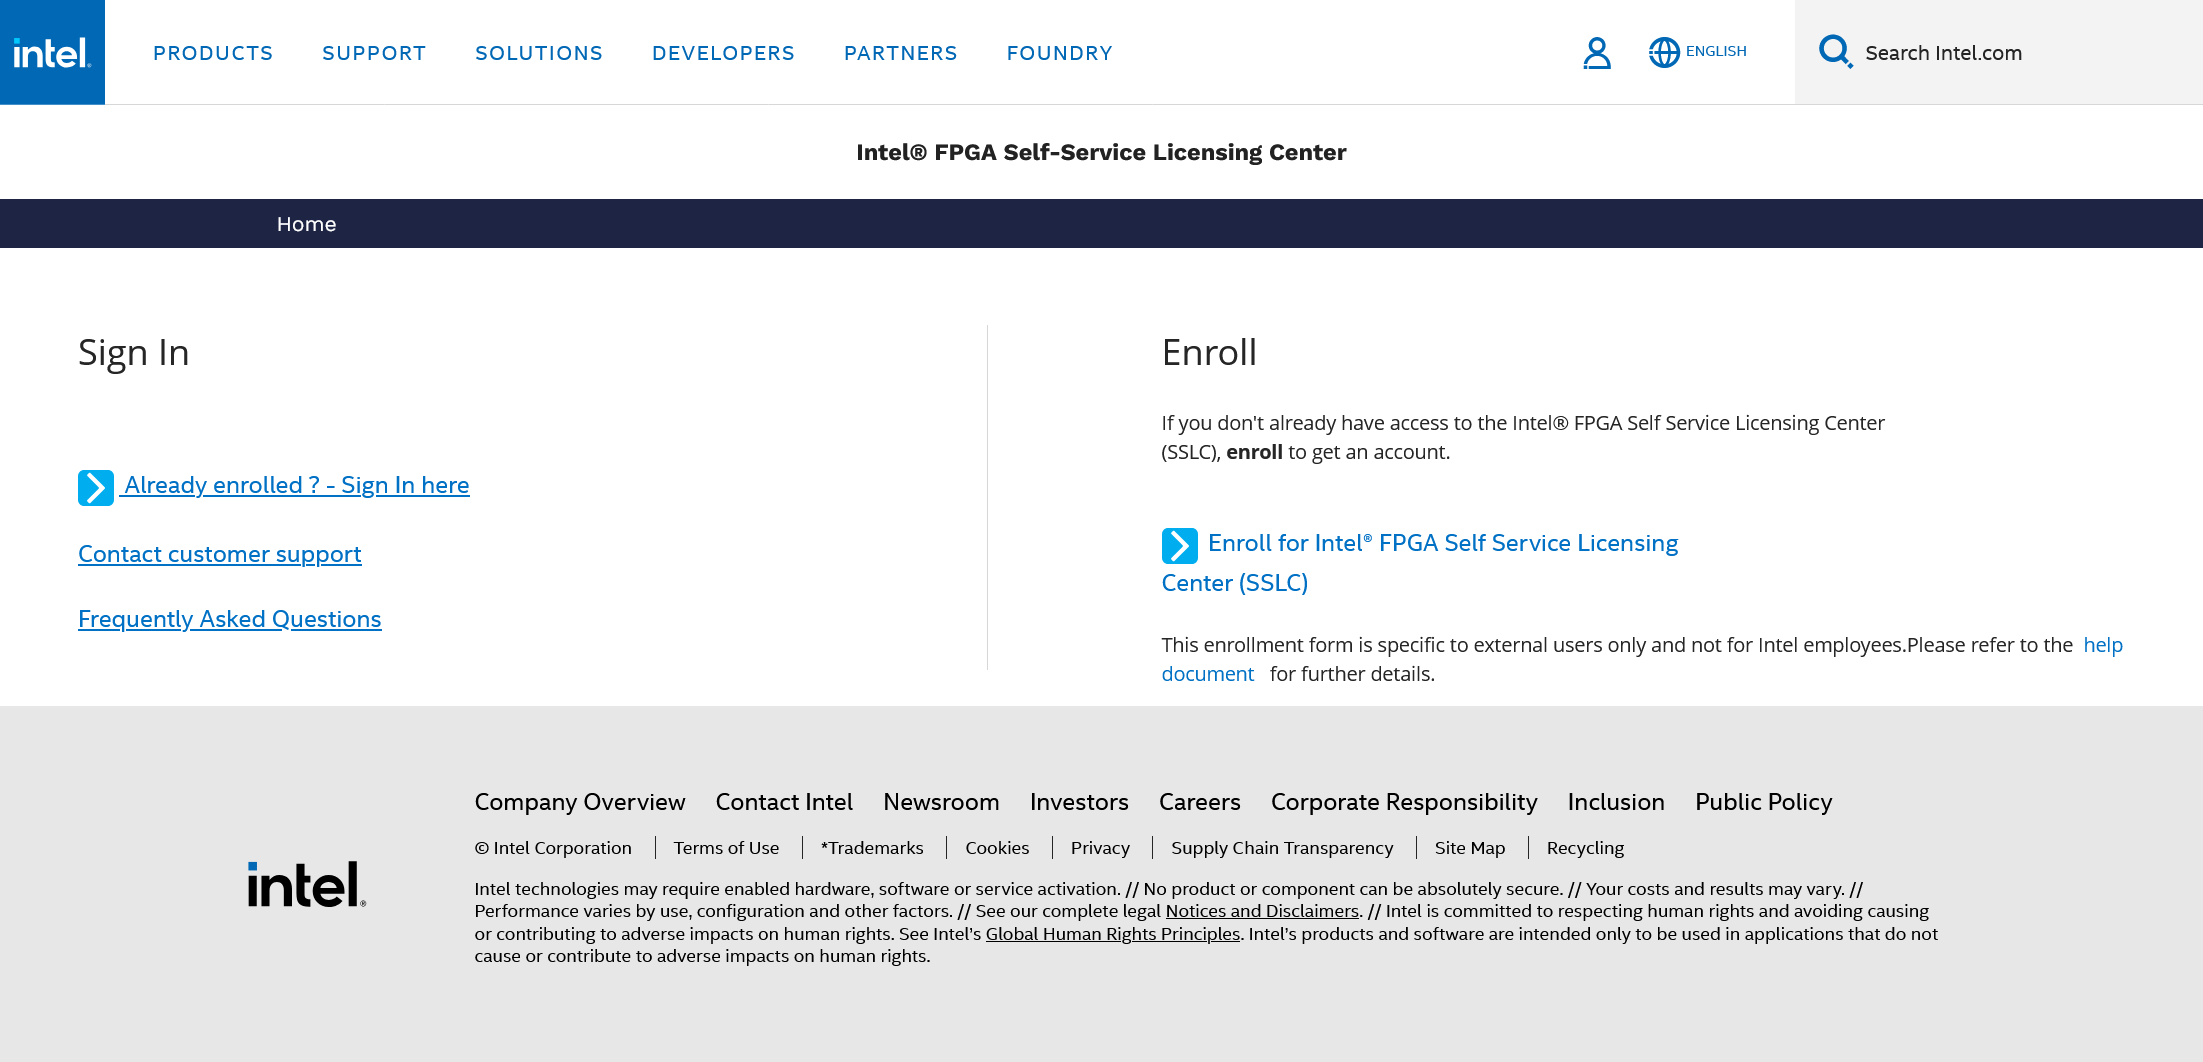
\includegraphics[width=\linewidth]{03_01_IntelLicensingPortalSignIn.png} \caption{Trang đăng nhập Cổng Intel Licensing Portal.} \label{fig:03_01} \end{figure}
\begin{figure}[htbp] \centering 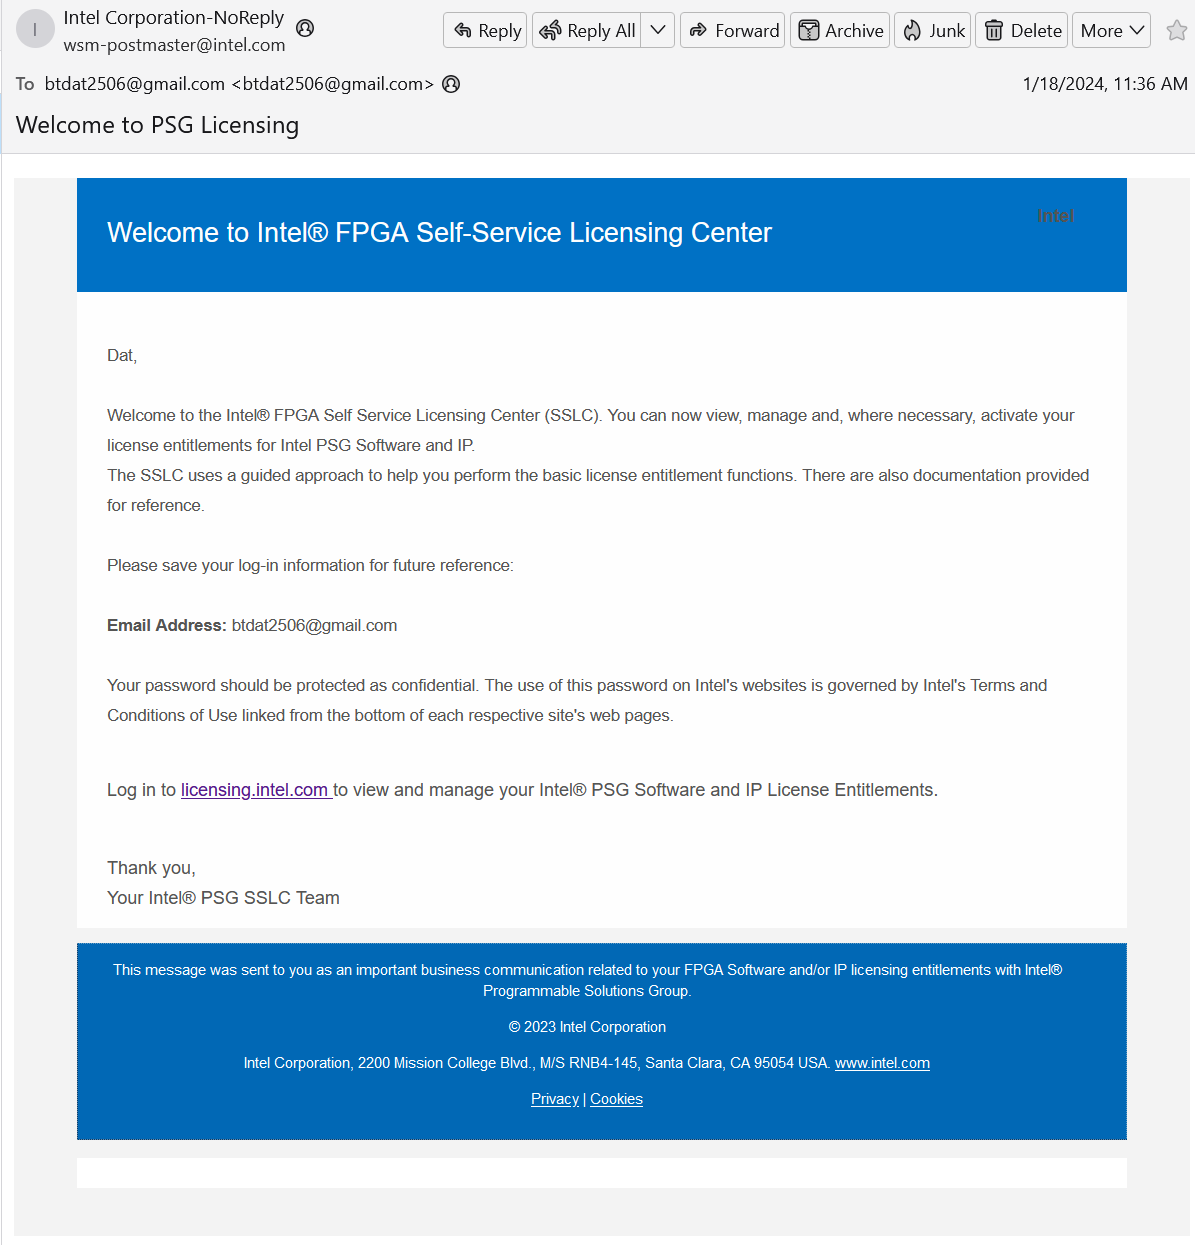
\includegraphics[width=\linewidth]{03_02_IntelLicensingWelcome.png} \caption{Email thông báo tài khoản Intel FPGA Self-Service Licensing đã được tạo thành công.} \label{fig:03_02} \end{figure}
\begin{figure}[htbp] \centering 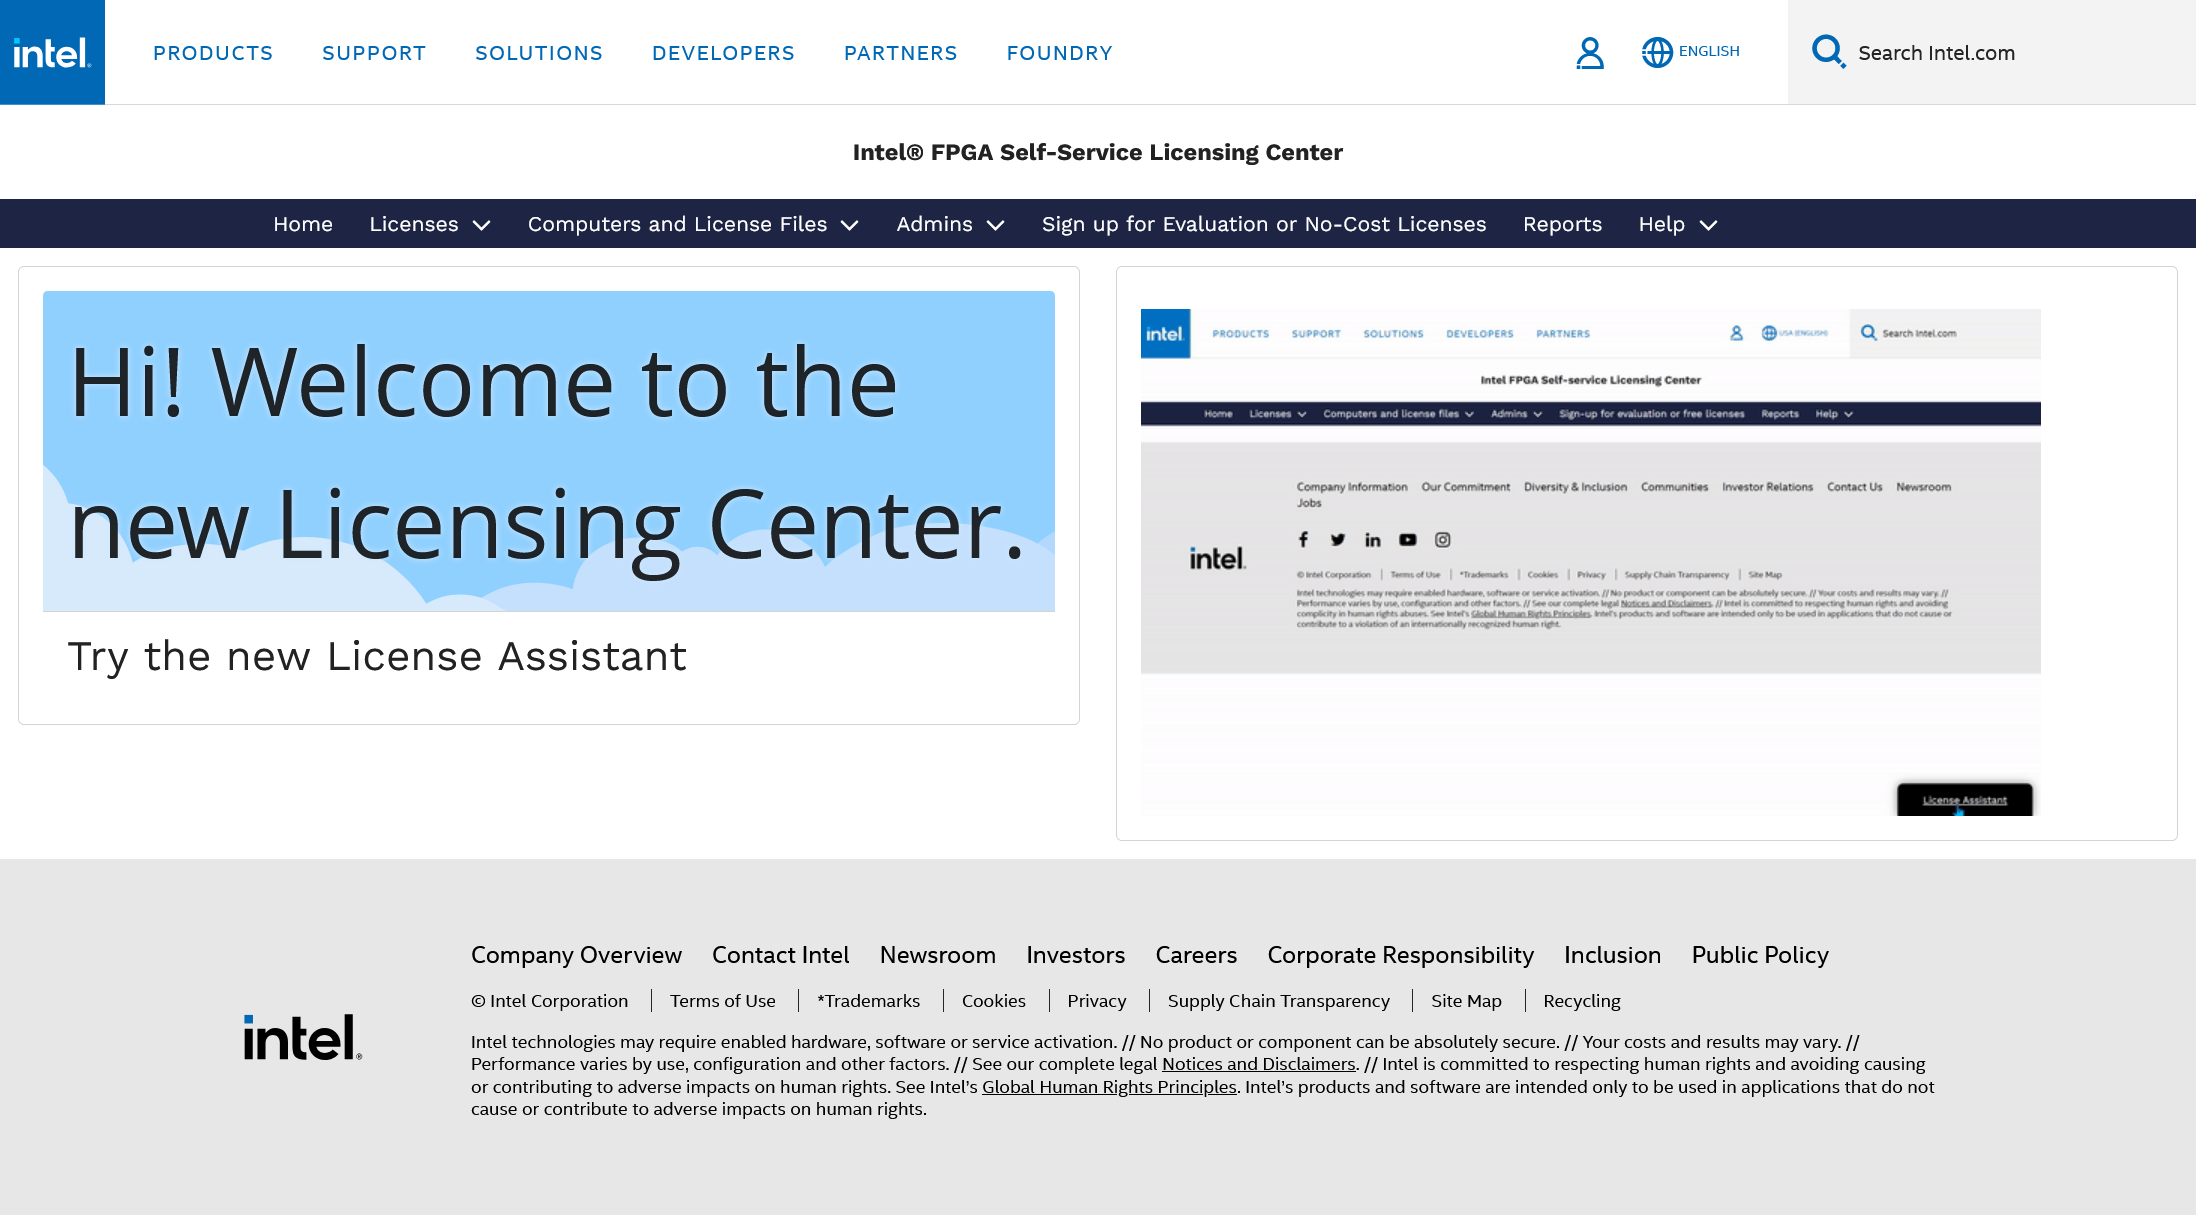
\includegraphics[width=0.9\linewidth]{03_03_IntelLicensingEvalSelection.png} \caption{Chọn "Sign up for Evaluation or No-Cost Licenses".} \label{fig:03_03} \end{figure}
\begin{figure}[htbp] \centering 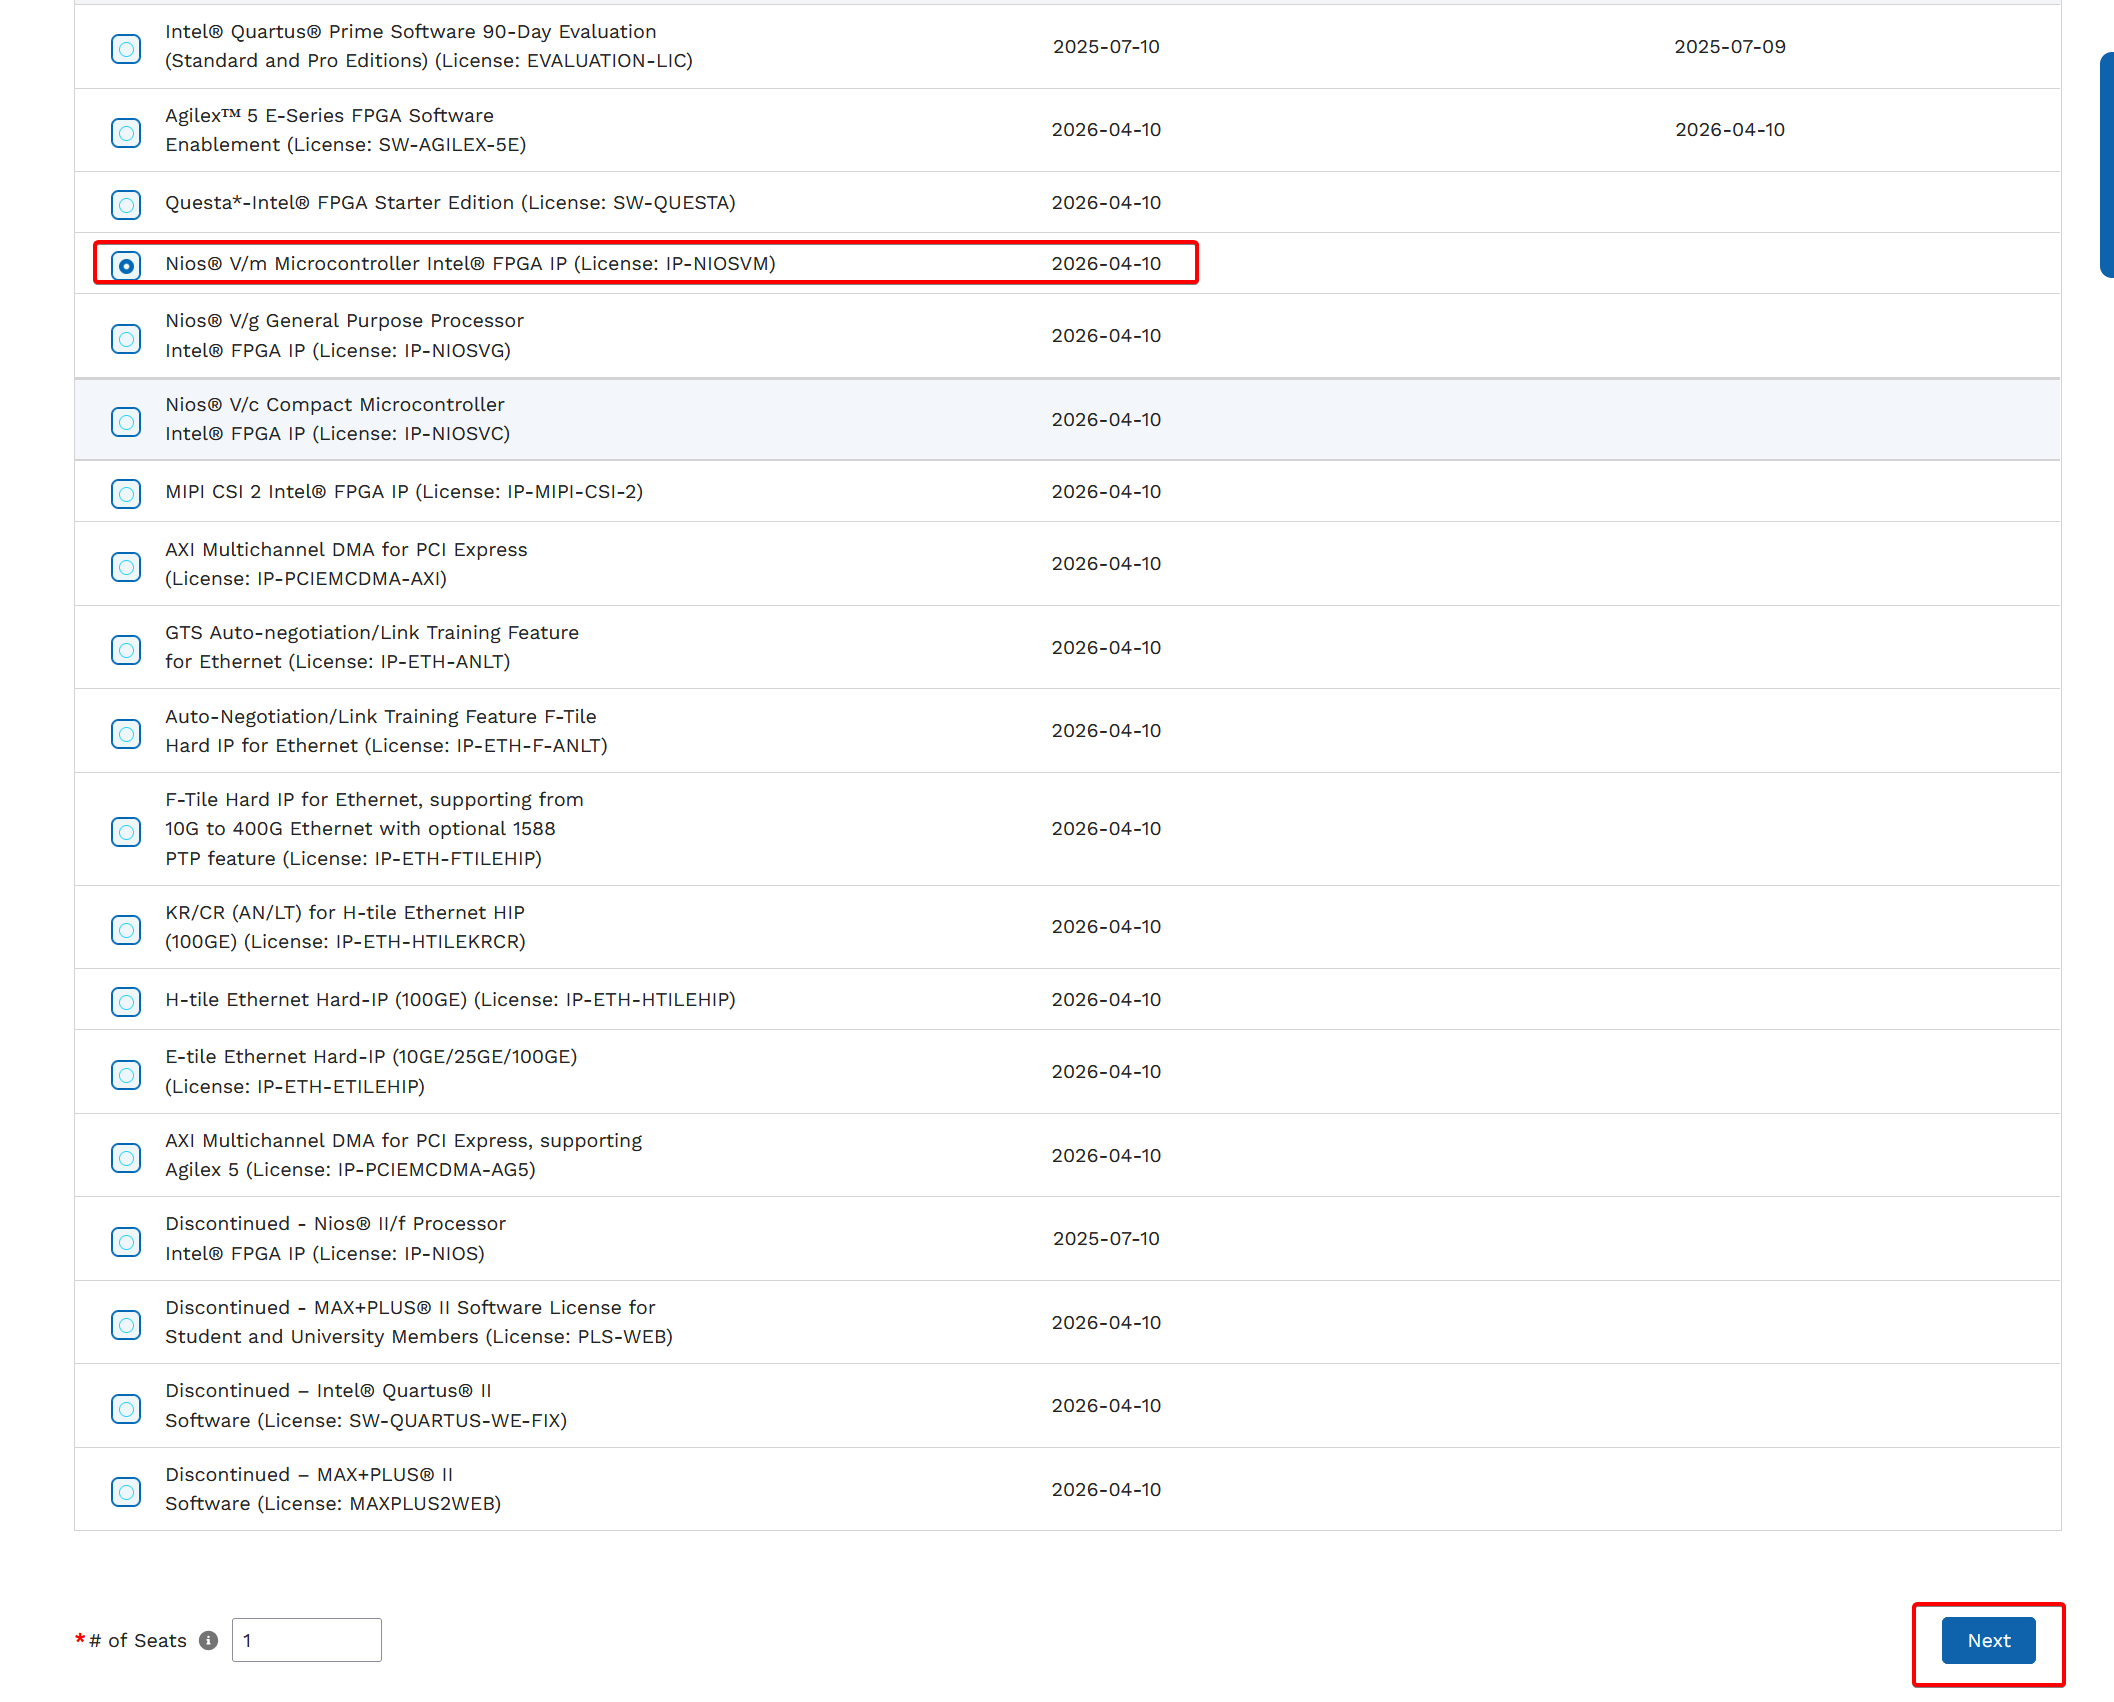
\includegraphics[width=\linewidth]{03_04_IntelLicensingNiosVSelection.png} \caption{Chọn bộ xử lý Nios V/m để cấp phép License.} \label{fig:03_04} \end{figure}
\begin{figure}[htbp] \centering 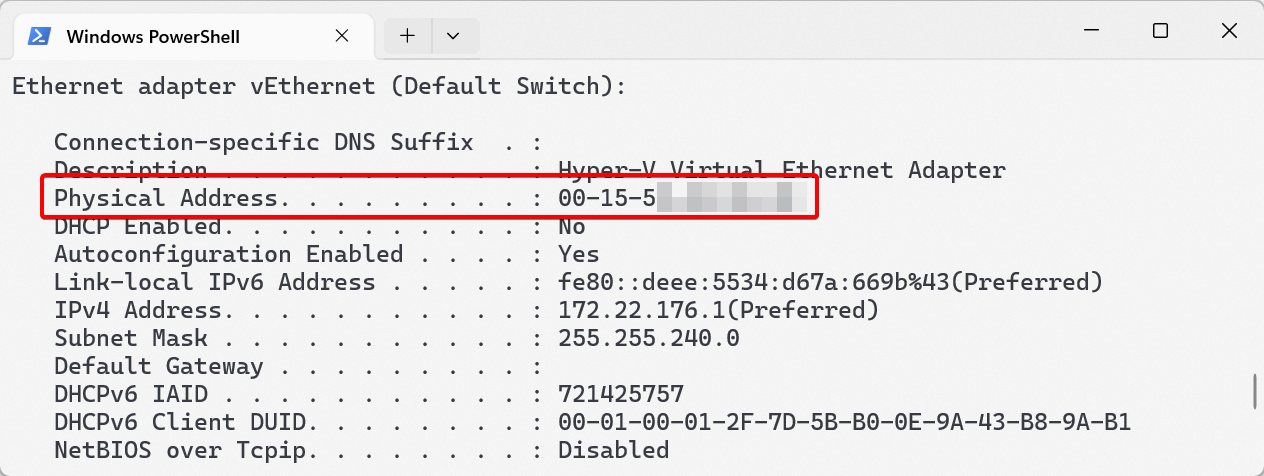
\includegraphics[width=0.8\linewidth]{03_05_IntelLicensingNICConfig.png} \caption{Tìm ID Card Giao diện Mạng (Network Interface Card - NIC ID) (Địa chỉ Vật lý).} \label{fig:03_05} \end{figure}
\begin{figure}[htbp] \centering 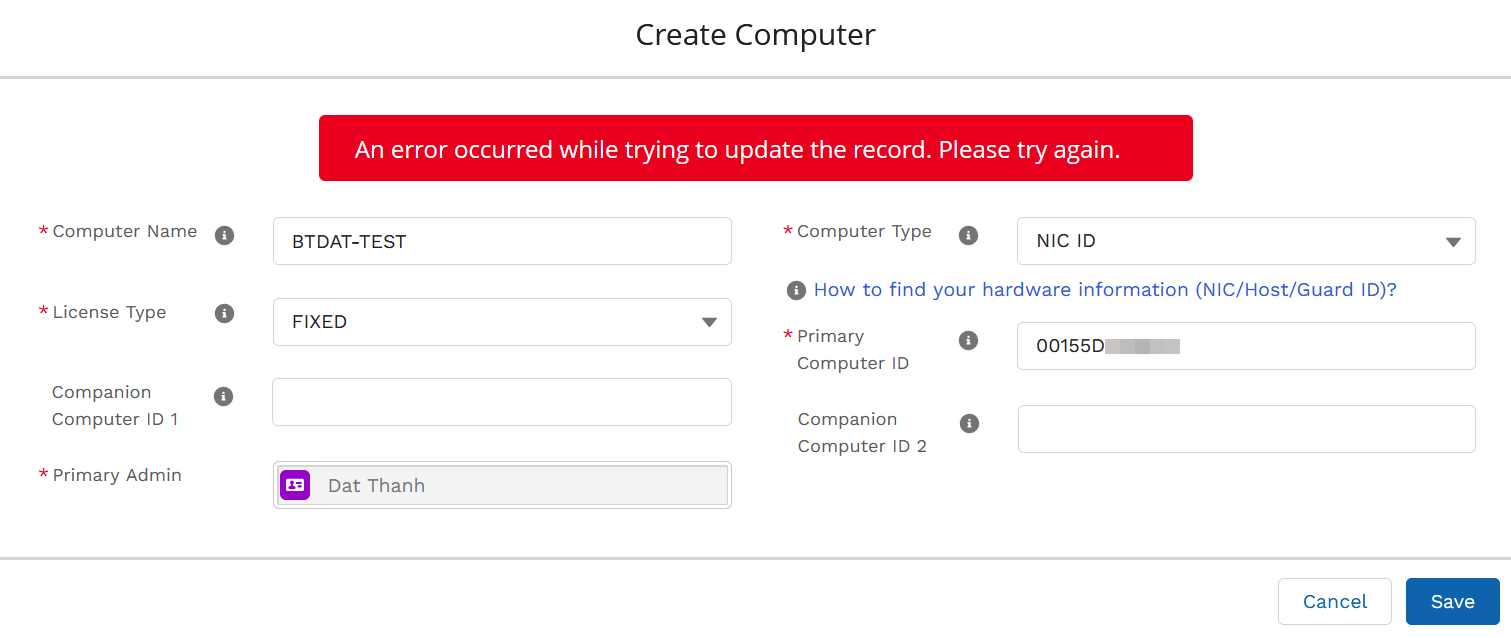
\includegraphics[width=0.8\linewidth]{03_06_IntelLicensingComputerInfo.png} \caption{Nhập thông tin máy tính (Tên, Loại, NIC ID) cho giấy phép.} \label{fig:03_06} \end{figure}
\begin{figure}[htbp] \centering 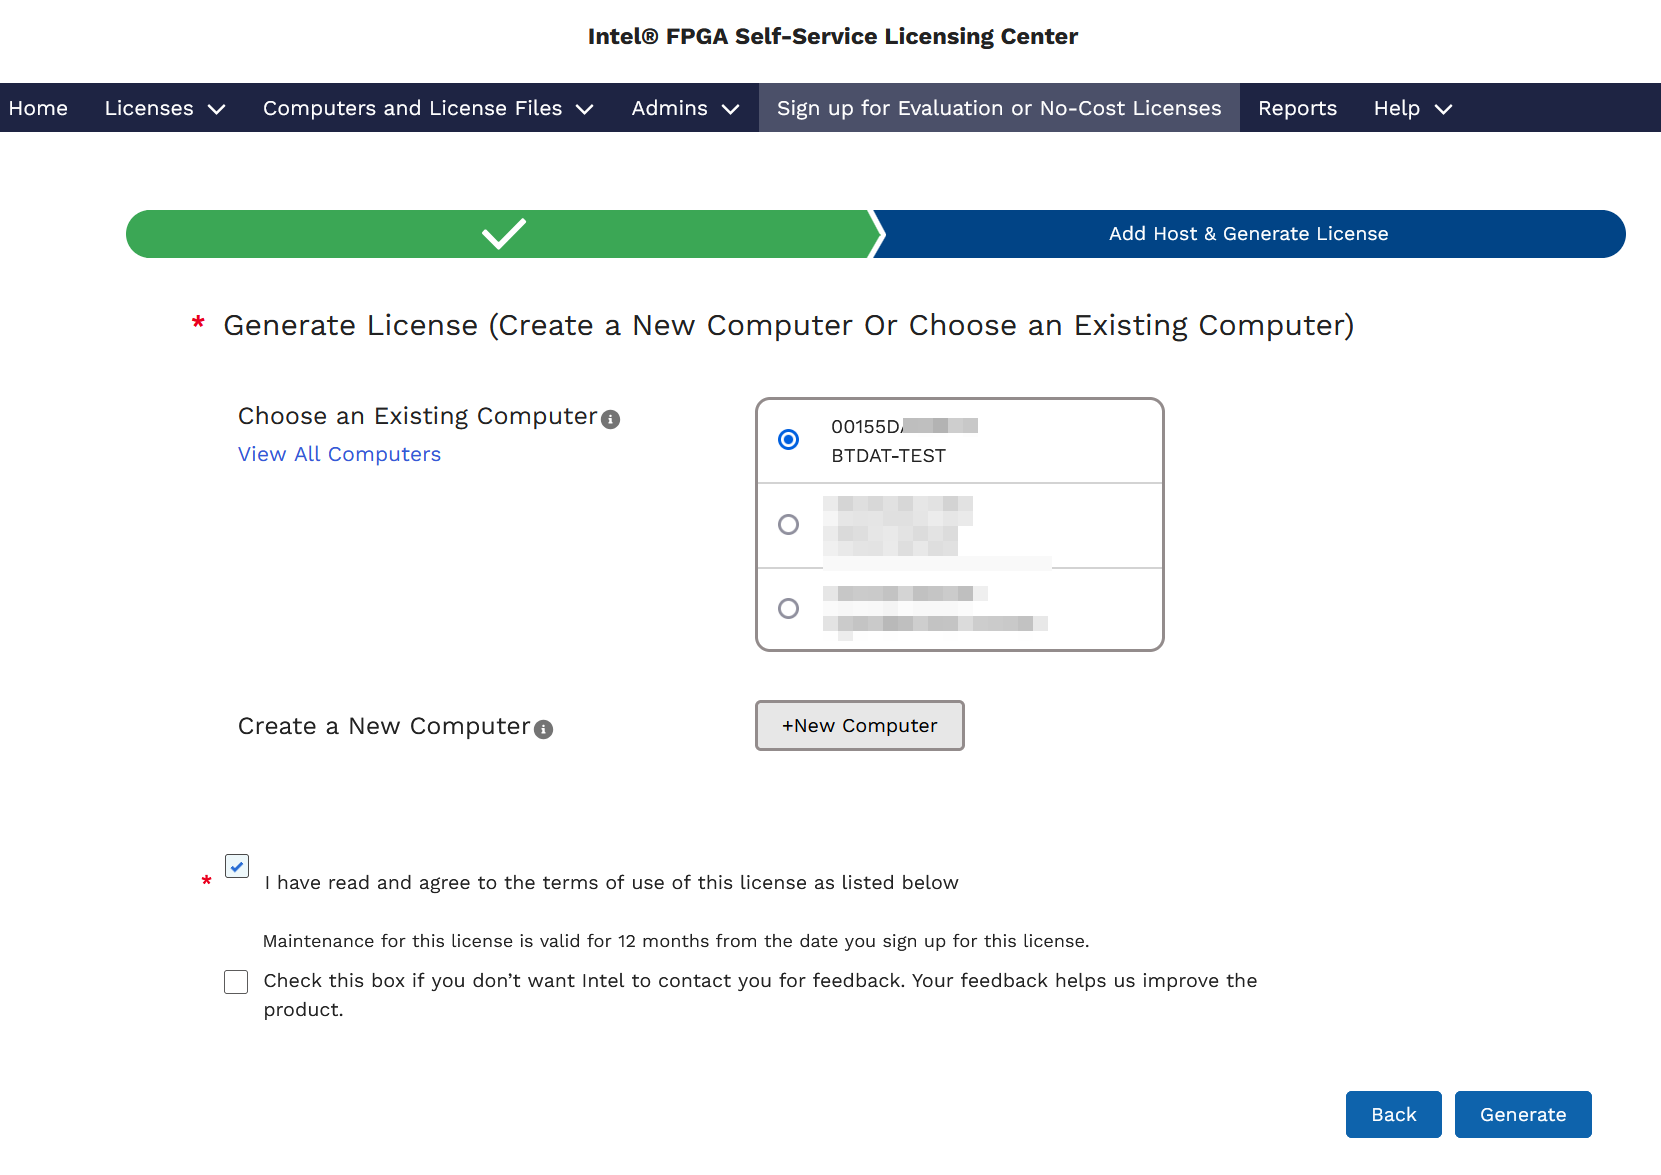
\includegraphics[width=0.8\linewidth]{03_07_IntelLicensingGenerate.png} \caption{Tạo giấy phép cố định (fixed license) dựa trên chi tiết máy tính.} \label{fig:03_07} \end{figure}
\begin{figure}[htbp] \centering 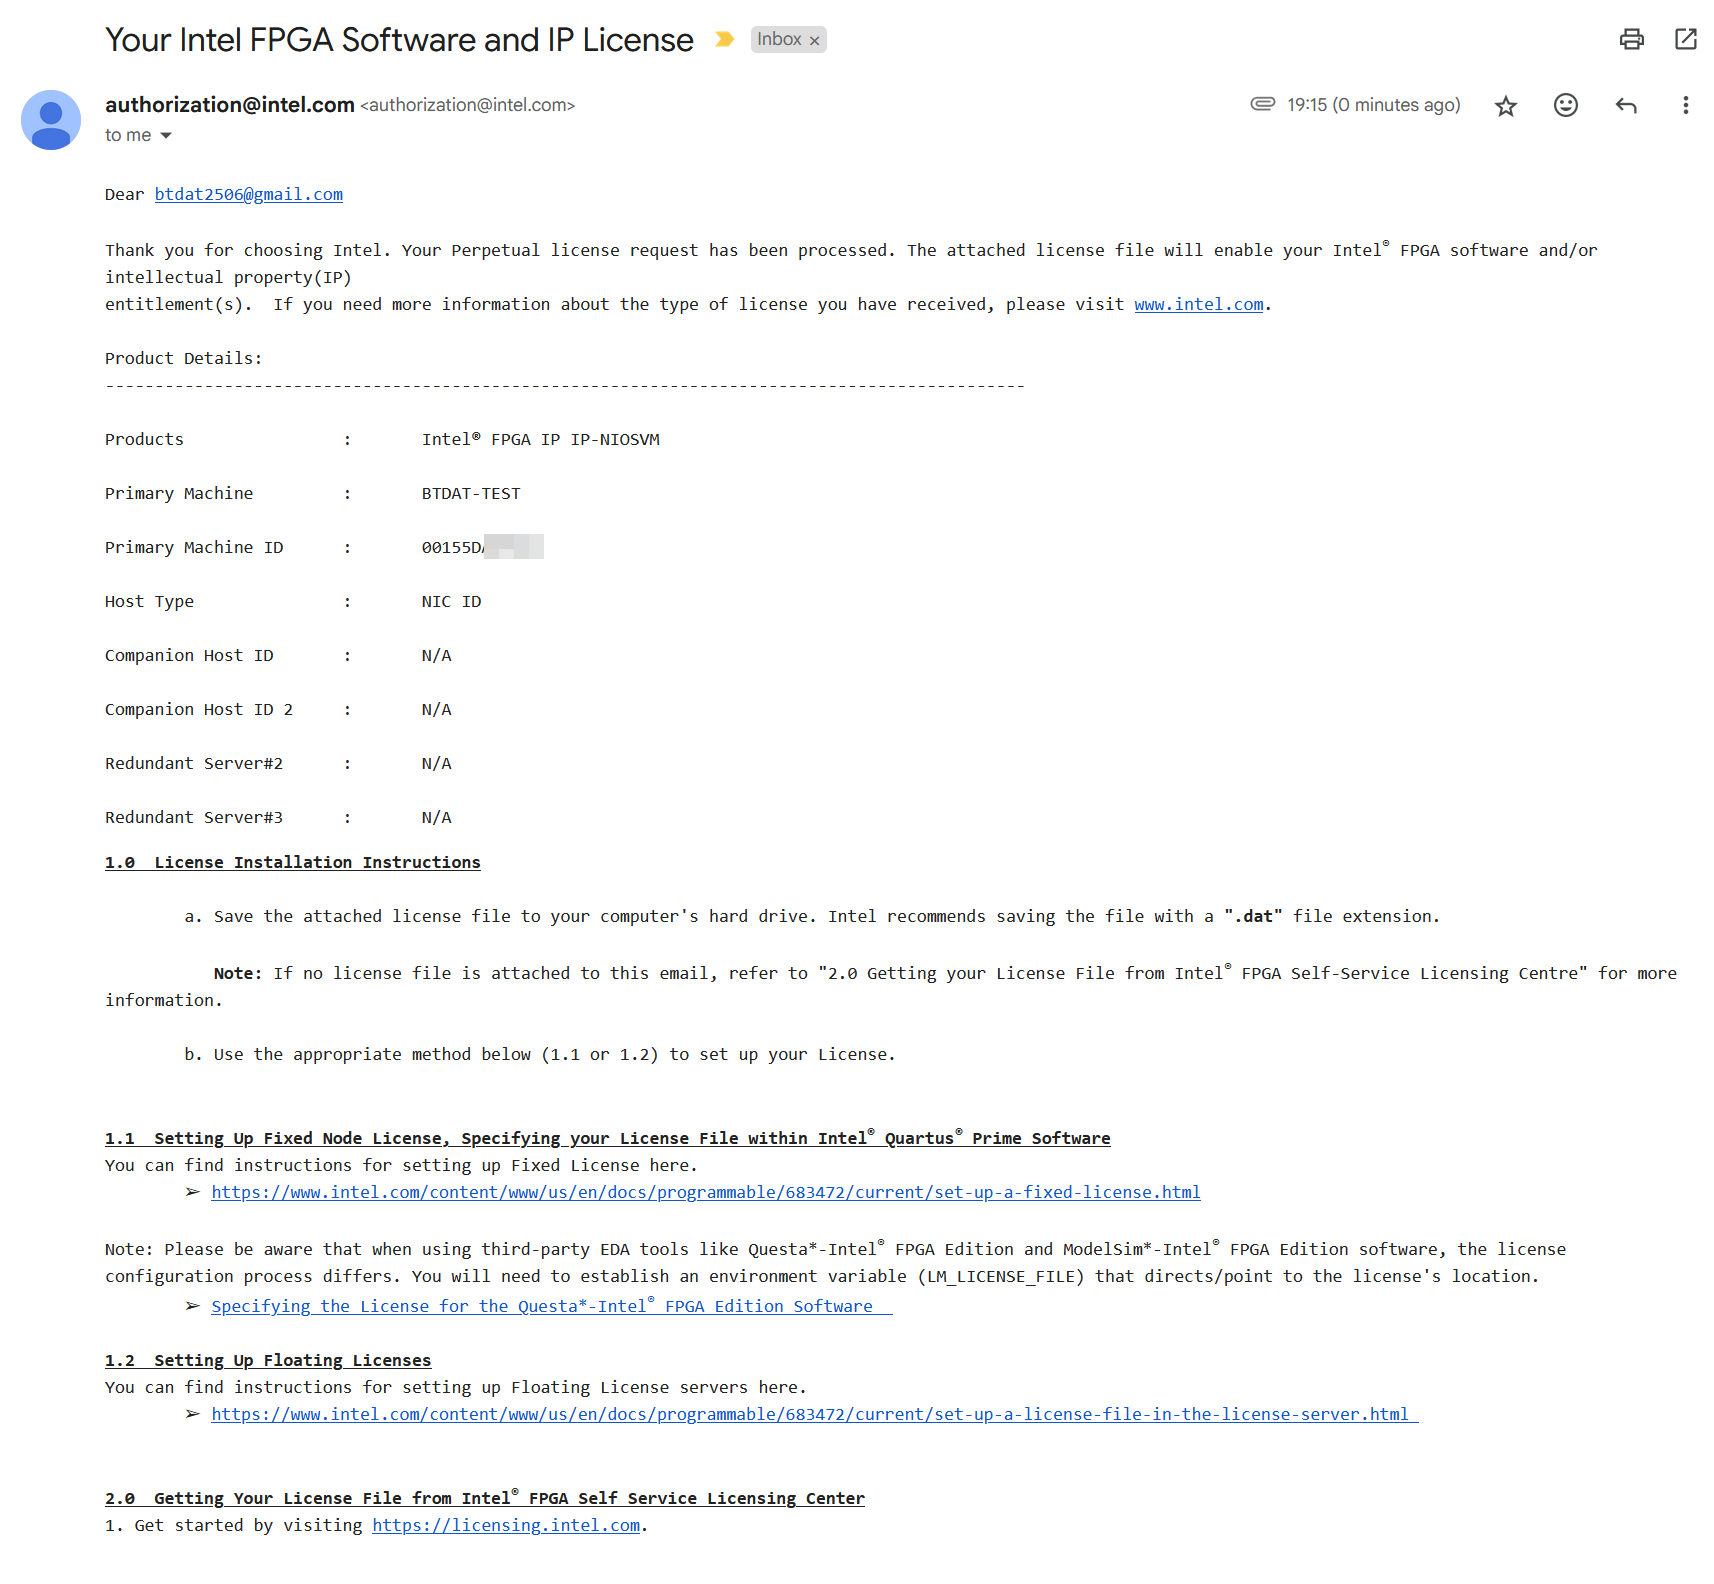
\includegraphics[width=\linewidth]{03_08_IntelLicenseEmailConfirmation.png} \caption{Email xác nhận chứa tệp giấy phép đính kèm.} \label{fig:03_08} \end{figure}
\begin{figure}[htbp] \centering 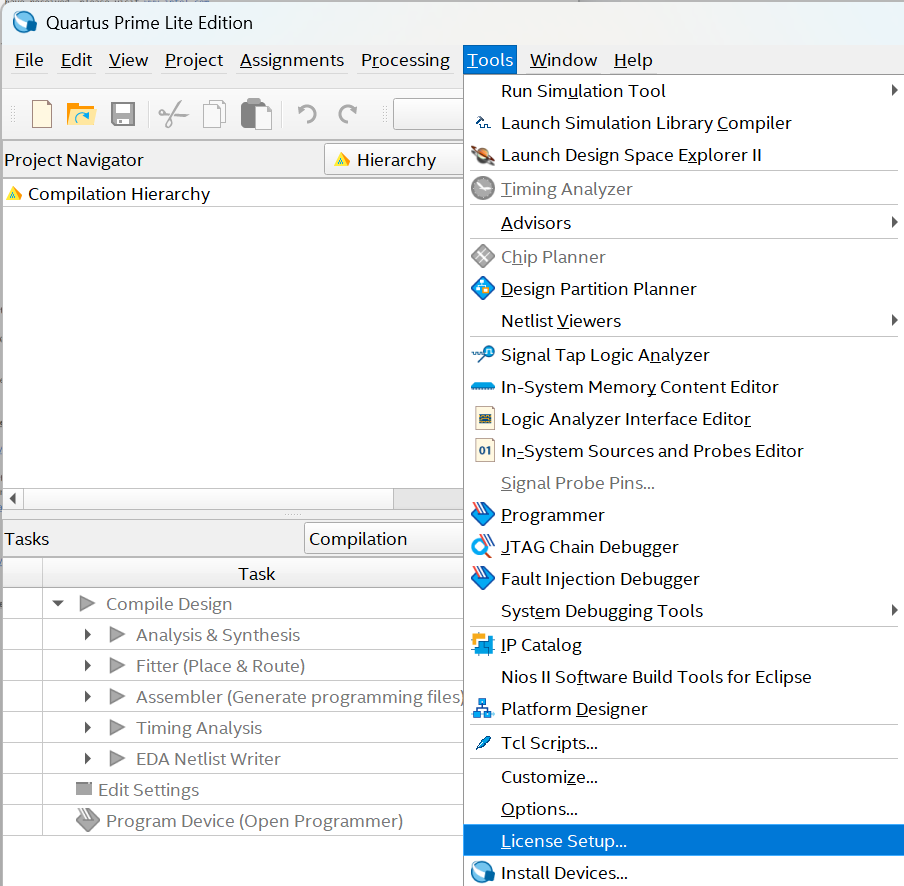
\includegraphics[width=0.65\linewidth]{03_09_QuartusToolsMenu.png} \caption{Truy cập Cài đặt Giấy phép (License Setup) từ menu Công cụ (Tools) của Quartus.} \label{fig:03_09} \end{figure}
\begin{figure}[htbp] \centering 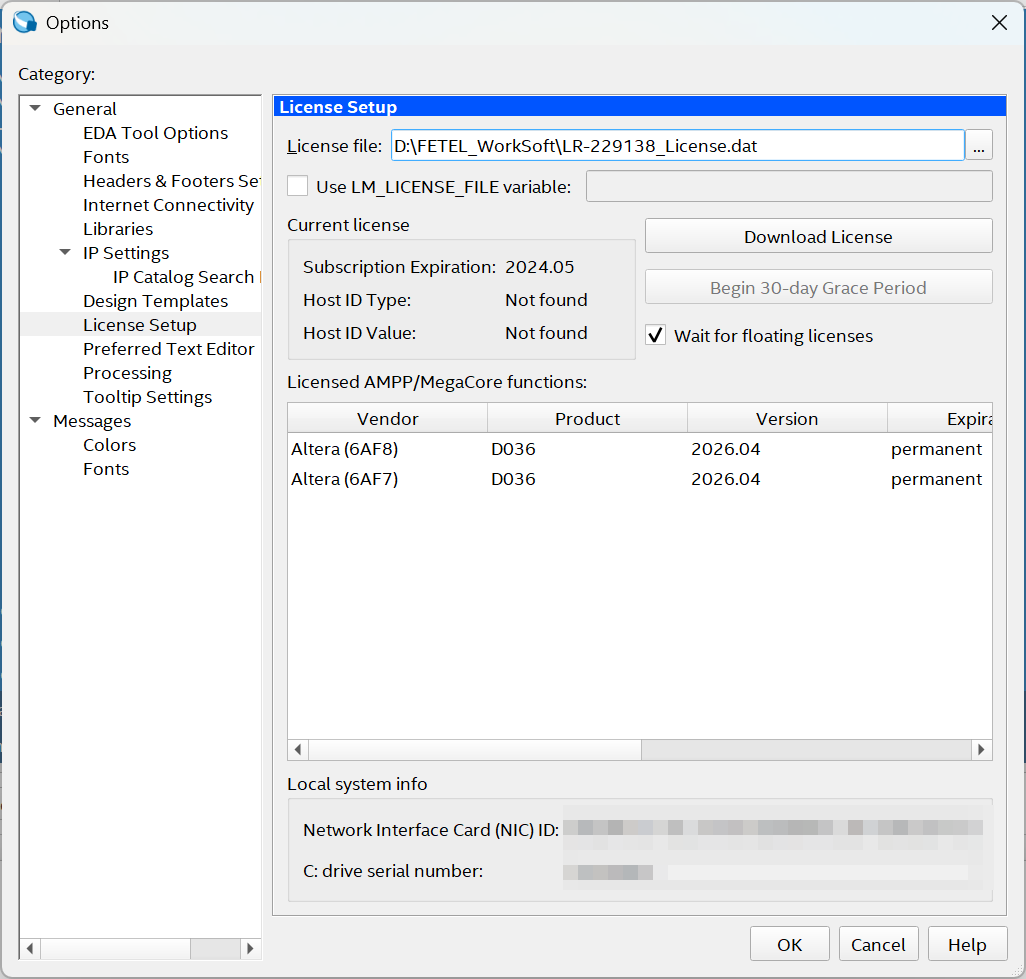
\includegraphics[width=0.65\linewidth]{03_10_QuartusLicenseSetup.png} \caption{Cửa sổ Cài đặt Giấy phép Quartus (Quartus License Setup) hiển thị tệp giấy phép Nios V/m đã thêm.} \label{fig:03_10} \end{figure}

